\section*{Eidesstattliche Erklärung}
Hiermit erkläre ich an Eides statt, dass ich die vorgelegte Diplomarbeit selbstständig und ohne Benutzung anderer als der angegebenen Hilfsmittel angefertigt habe. Gedanken, die aus fremden Quellen direkt oder indirekt übernommen wurden, sind als solche gekennzeichnet.

Die Arbeit wurde bisher in gleicher oder ähnlicher Weise keiner anderen Prüfungsbehörde vorgelegt und auch noch nicht veröffentlicht. \\[1em]
Leonding, am \duedatede \\[5em]
\ifthenelse{\isundefined{\firstauthor}}{}{\firstauthor}
\ifthenelse{\isundefined{\secondauthor}}{}{\kern-1ex, \secondauthor} \\[5em]


\begin{otherlanguage}{english}
\section*{Declaration of Academic Honesty}
Hereby, I declare that I have composed the presented paper independently on my own and without any other resources than the ones indicated. All thoughts taken directly or indirectly from external sources are properly denoted as such.

This paper has neither been previously submitted to another authority nor has it been published yet. \\[1em]
Leonding, \duedateen \\[5em]
\ifthenelse{\isundefined{\firstauthor}}{}{\firstauthor}
\ifthenelse{\isundefined{\secondauthor}}{}{\kern-1ex, \secondauthor}
\end{otherlanguage}


\begin{abstract}
	\begin{itemize}
		\item {\em Aufgabenstellung} \\ Um den Kunden der Firma {\projectpartner} die Visualisierung eines für sie designten Bades zu erleichtern, ist es notwendig, ihnen eine möglichst genaue und detaillierte Darstellung anzubieten. Dies bezieht sich sowohl auf das Design, die Komponenten als auch für die Bauanleitung. Da nicht nur die Hotelketten das Modell zu Gesicht bekommen, sondern auch Monteure, die sich daran beim Zusammenbauen orientieren können. Dadurch dass der Fortschritt und das fertige Bad aus verschiedenen Perspektiven angesehen werden kann, wird die Vision für alle klarer und einfacher. Da die ganze Applikation webbasiert ist, ist sie plattformunabhängig und kann dank Electron lokal und ohne Internet ausgeführt werden. Bisher wurde dies immer mit Präsentationsvideos umgesetzt, die jedoch sehr unflexibel sind und zeitintensiv waren. Die Probleme waren dabei, dass das Bad immer nur aus einer Perspektive zu sehen war, das Modell nicht interaktiv war und Kundenwünsche nicht sofort umgesetzt werden konnten. Der Umgang mit dem Tool wird möglichst intuitiv erfolgen und besondere Ressourcenanforderungen sind nicht präsent.
		\item {\em Umsetzung} \\ Die Web-Anwendung basiert auf den gängigen Technologien HTML, JavaScript, Three.js und WEB.GL. Dies ermöglicht es über einen beliebigen Browser und beliebiges Betriebssystem darauf zuzugreifen. Die einzige Anforderung ist eine Internetverbindung. Die Wahl für die oben genannten Technologien ist darauf zurückzuführen, dass alle robust, zukunftssicher, gut dokumentiert und weitverbreitet sind. Damit eignen sie sich perfekt für die Applikation und sind ein wichtiger Beitrag dafür das die Anwendung wartbar ist und bleibt.
		\item {\em Ergebnisse} \\ Die Software wurde nach Abschluss der Arbeit an das Unternehmen {\projectpartner} übergeben. Demonstrationen und Tutorials an die zukünftigen Anwender wurden durch das Entwicklerteam durchgeführt. Unter folgender Adresse \url{http://vm85.htl-leonding.ac.at/} kann die Diplomarbeit begutachtet und verwendet werden.
	\end{itemize}
\clearpage \newpage	
	
\begin{figure}[h]
    \centering
    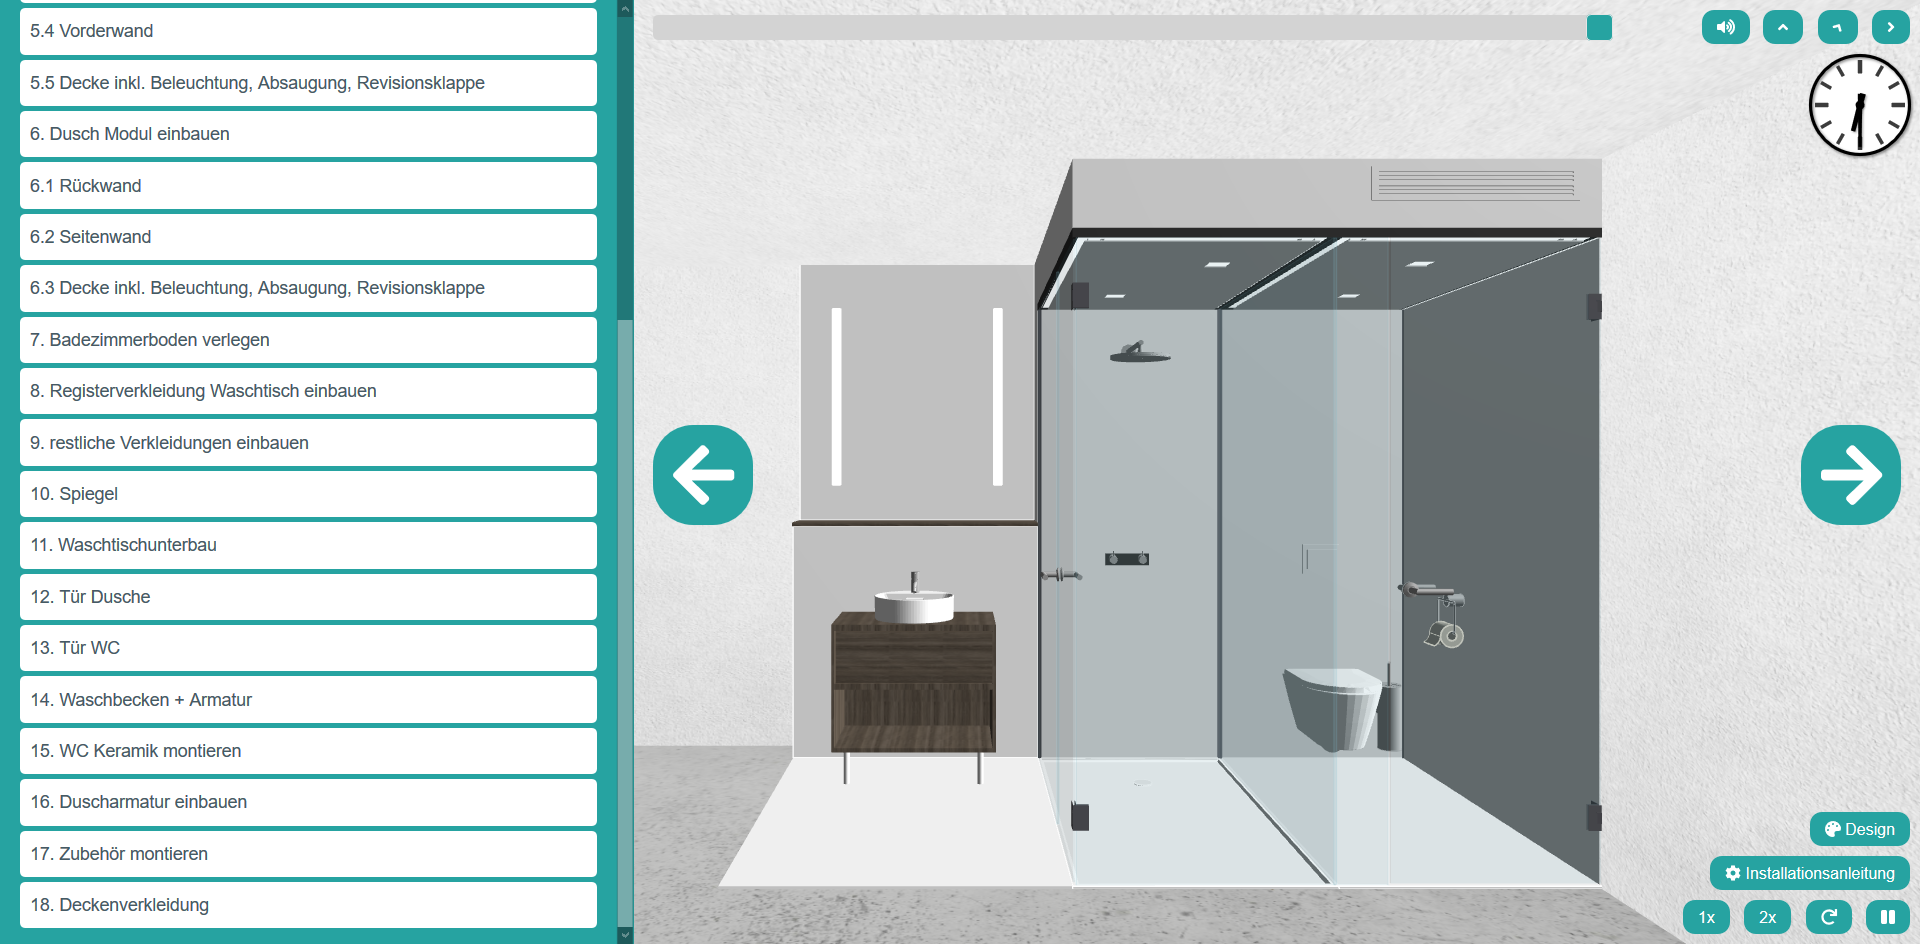
\includegraphics[width=0.65\linewidth]{images/Screenshot_front.png}
			\caption{Bad Designer; Frontalansicht}
\end{figure}

	
\begin{figure}[h]
    \centering
    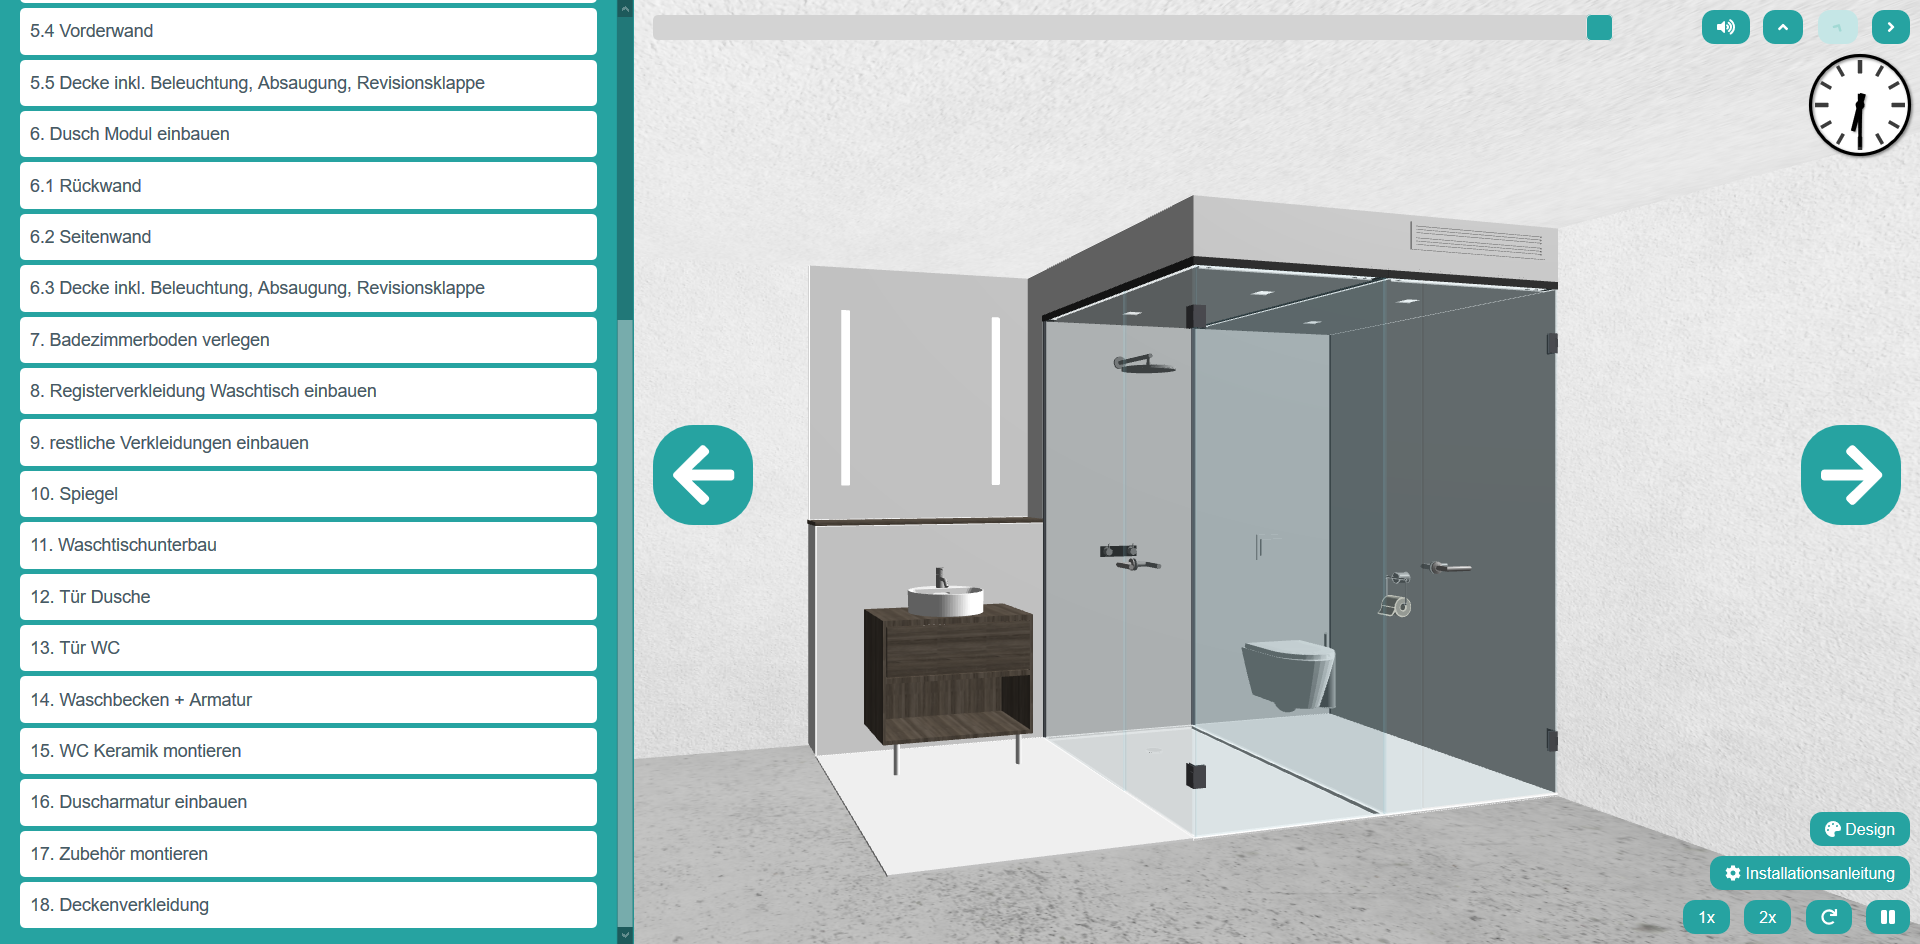
\includegraphics[width=0.65\linewidth]{images/Screenshot_schraeg.png}
	\caption{Bad Designer; Schrägansicht}
\end{figure}	


\begin{figure}[h]
    \centering
    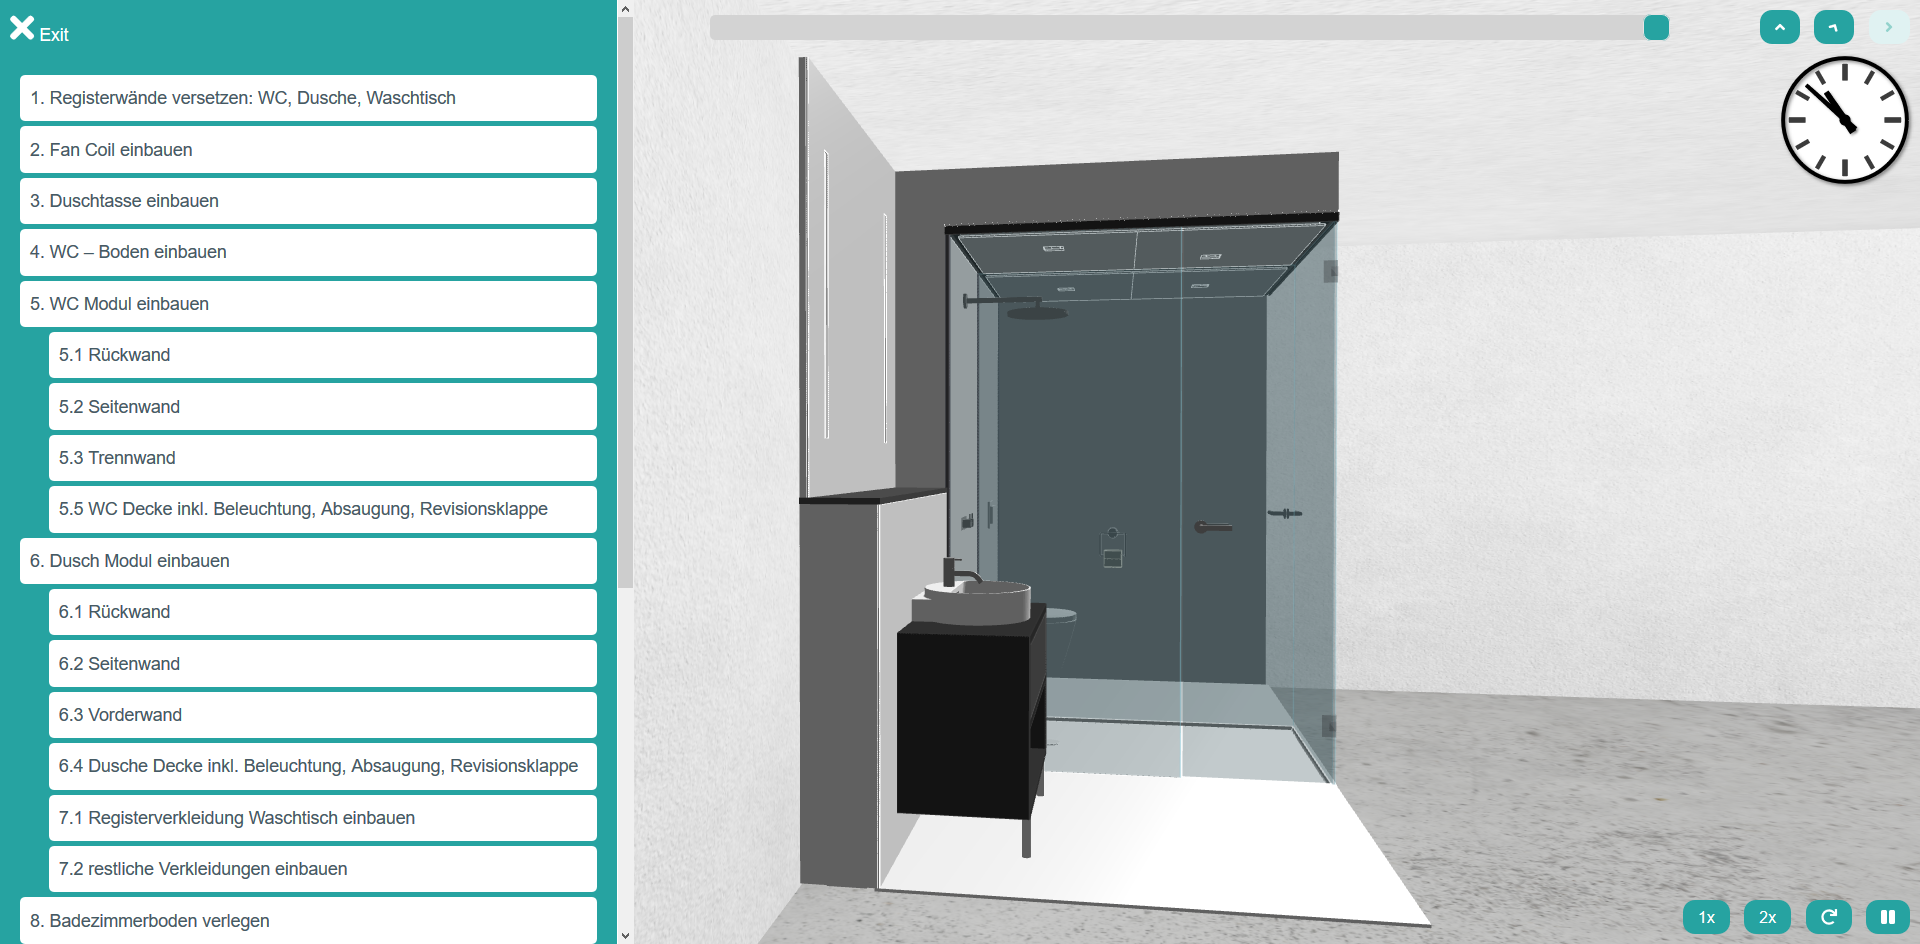
\includegraphics[width=0.65\linewidth]{images/Screenshot_seite.png}
	\caption{Bad Designer; Seitenansicht}
\end{figure}

\end{abstract}

	\newpage
	\clearpage
\begin{otherlanguage}{english}
\begin{abstract}

% \begin{enumerate}
\begin{itemize}
	\item {\em Definition of the project} \\ In order to present the customers of {\projectpartner} a visualization of a custom-made modular bath it is necessary to have a precise and detailed illustration. This is especially important for the custom design, the components and for the construction manual. As the model will be showed to the assembler as well it is important that it is possible to build it with the manual the application provides. The progress and the complete bath can be viewed from multiple angles with the intention of making the concept clearer and simpler for all. As it is a web application it can be run on every operating system and thanks to Electron locally runable without an internet connection. Up to now this was done with presentation videos, but they were too inflexible and time-consuming. Moreover, the bath was only visible from one angle, the model was not interactive and customer requirements could not be implemented immediately. The tool is as intuitive as possible and does not require special resources.
	
	\item {\em Implementation} \\ The web-app is based on the commonly used technologies HTML, JavaScript, Three.js and WebGL. This allows it to be run on every operating system and any modern browser. It only requires a internet connection. The mentioned technologies were uses because they are all robust, future-proof, well documented and extendable. Thanks to these attributes they are perfect fit for the application and make it easier to service.
	
	\item {\em Results} \\ The software was delivered after the thesis to the company {\projectpartner}. Demonstrations and tutorials were provided to the future users by the developing team. The work is publicly accessible on this website \url{http://vm85.htl-leonding.ac.at/}.
\end{itemize}

\clearpage \newpage

\begin{figure}[h]
    \centering
    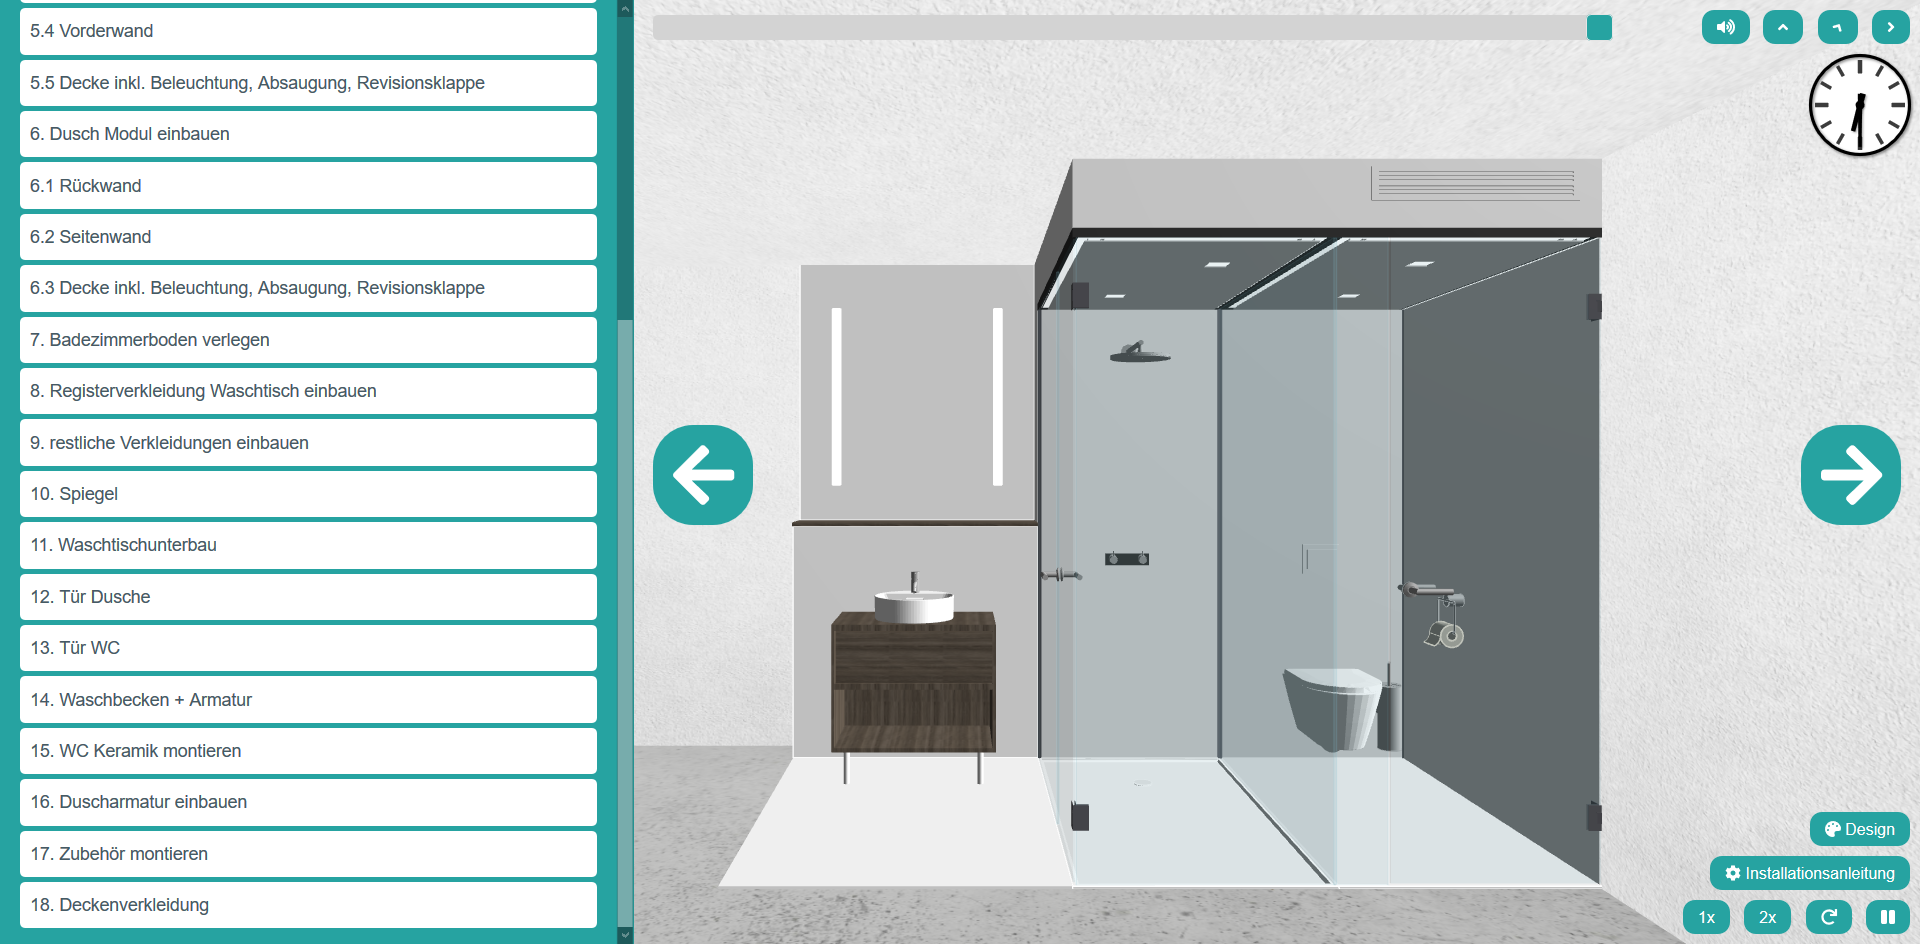
\includegraphics[width=0.65\textwidth]{images/Screenshot_front.png}
		\caption{Bad Designer; Frontal view}
\end{figure}



\begin{figure}[h]
    \centering
    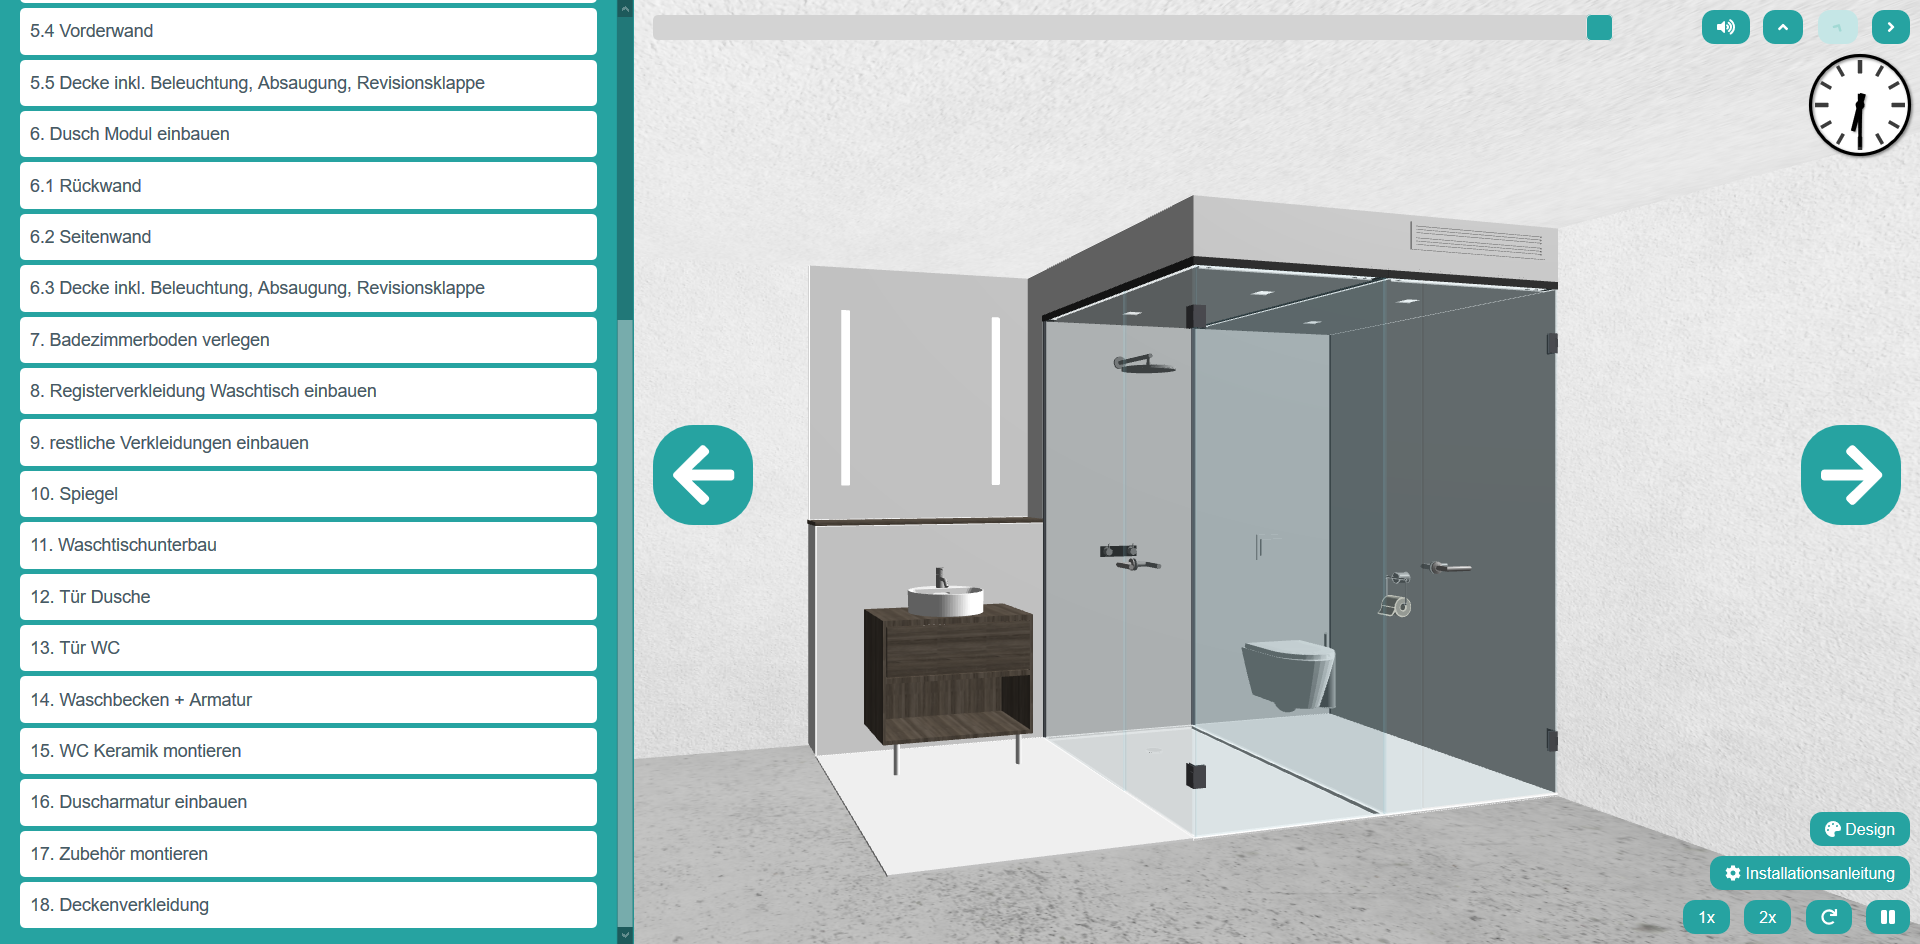
\includegraphics[width=0.65\textwidth]{images/Screenshot_schraeg.png}
		\caption{Bad Designer; Oblique view }
\end{figure}


\begin{figure}[h]
    \centering
    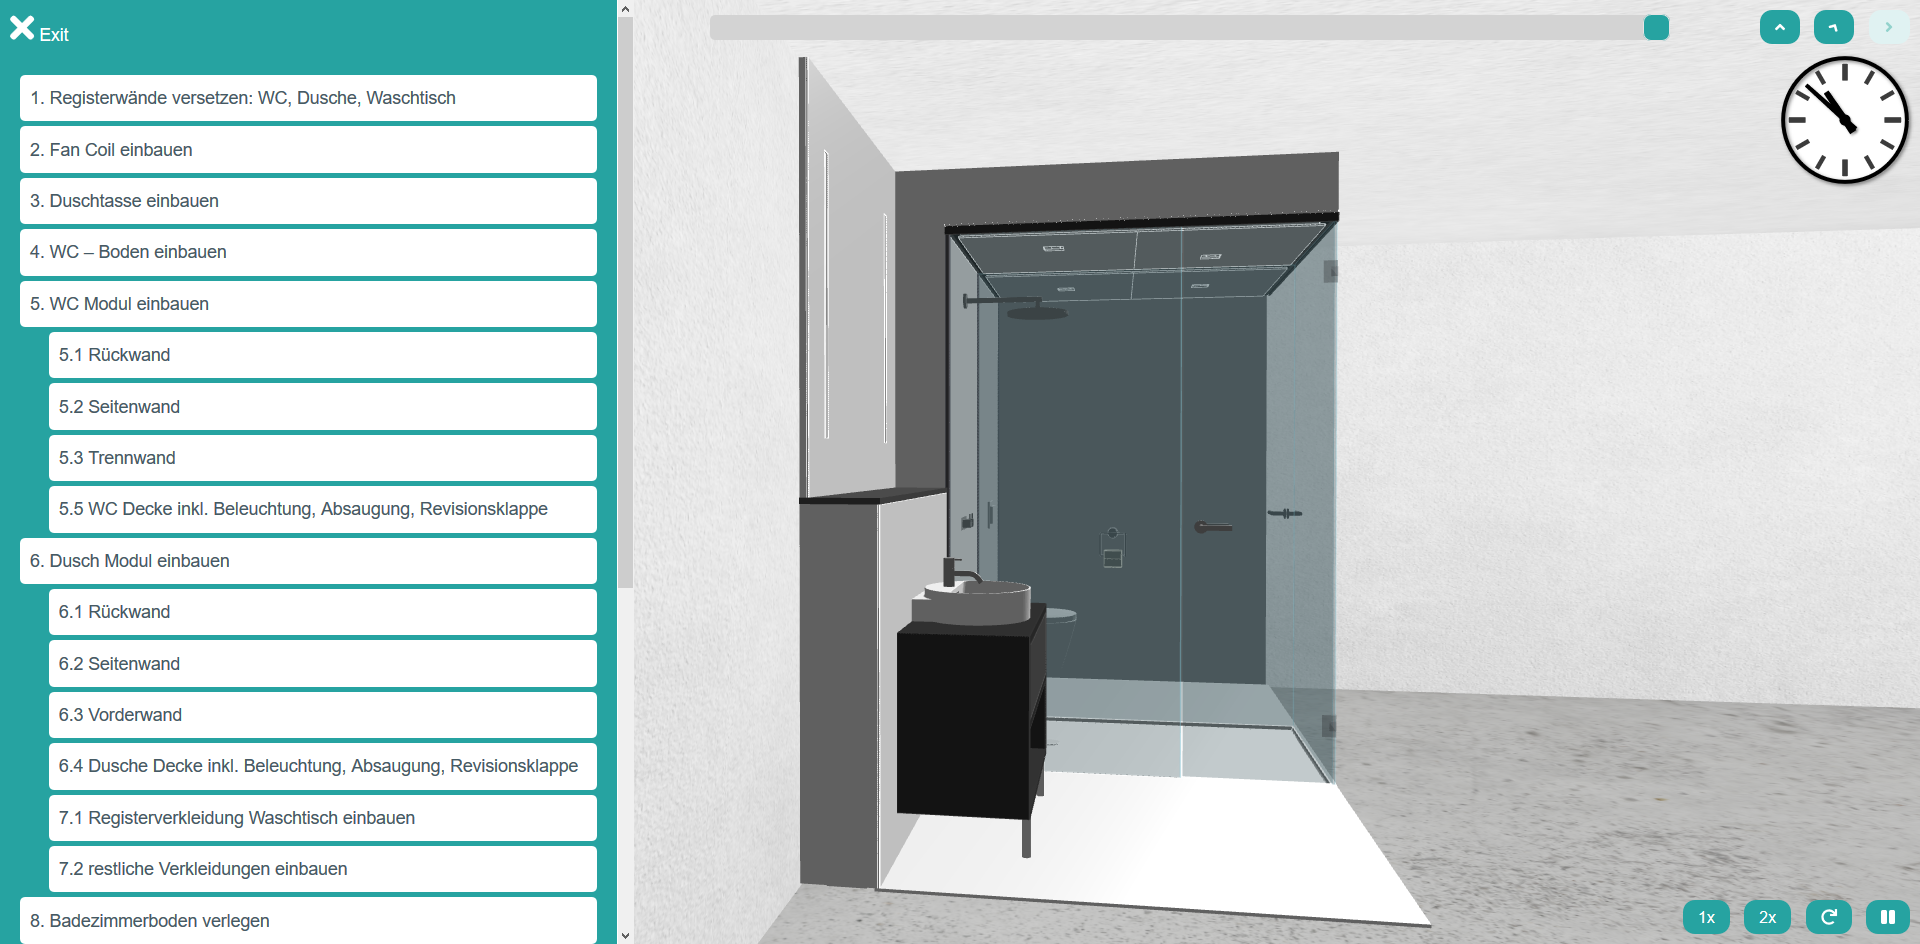
\includegraphics[width=0.65\textwidth]{images/Screenshot_seite.png}
		\caption{Bad Designer; Side view}
\end{figure}

\end{abstract}
\end{otherlanguage}

\newpage
\clearpage
\section*{Danksagungen}
Wir möchten uns sehr herzlich bei unserem Diplomarbeitsbetreuer {\supervisor} bedanken der uns stets fachlich und persönlich unterstützt hat und immer an unserer Seite stand. Einen großen Dank möchten wir auch an unseren Auftraggeber die {\projectpartner} richten die uns das Vertrauen geschenkt hat. Für das Vermitteln der Diplomarbeit möchten wir uns bei Prof. Dipl.-Ing. Richard Kainerstorfer bedanken.
\\ \\
Ein großer Dank gilt auch unseren Familien und Freunden die in der Zeit der Erstellung dieser Arbeit für uns da waren und uns unterstützt haben.